\documentclass[
]{jss}

\usepackage[utf8]{inputenc}

\providecommand{\tightlist}{%
  \setlength{\itemsep}{0pt}\setlength{\parskip}{0pt}}

\author{
\\
}
\title{}

\Plainauthor{}

\Abstract{

}


%% publication information
%% \Volume{50}
%% \Issue{9}
%% \Month{June}
%% \Year{2012}
%% \Submitdate{}
%% \Acceptdate{2012-06-04}

\Address{
  }


% Pandoc header
\usepackage{animate}



\begin{document}

\hypertarget{introduction}{%
\section{Introduction}\label{introduction}}

\begin{itemize}
\tightlist
\item
  This is an \textbf{R Markdown} document \citep{R-rmarkdown}.
\item
  Markdown is a simple formatting syntax for authoring HTML, PDF, and MS
  Word documents, etc.
\item
  For more details on using R Markdown, see
  \url{https://rmarkdown.rstudio.com}.
\end{itemize}

\hypertarget{r-markdown}{%
\section{R Markdown}\label{r-markdown}}

\hypertarget{embed-r-code}{%
\subsection{Embed R code}\label{embed-r-code}}

\hypertarget{data}{%
\subsubsection{Data}\label{data}}

You can embed an R code chunk like this:

\begin{CodeChunk}

\begin{CodeInput}
R> dat <- iris[, 1:2]
R> names(dat) <- c('x', 'y')
R> str(dat)
\end{CodeInput}

\begin{CodeOutput}
'data.frame':   150 obs. of  2 variables:
 $ x: num  5.1 4.9 4.7 4.6 5 5.4 4.6 5 4.4 4.9 ...
 $ y: num  3.5 3 3.2 3.1 3.6 3.9 3.4 3.4 2.9 3.1 ...
\end{CodeOutput}
\end{CodeChunk}

\hypertarget{draw-plots}{%
\subsection{Draw plots}\label{draw-plots}}

\hypertarget{starry-night}{%
\subsubsection{Starry night}\label{starry-night}}

\begin{CodeChunk}

\begin{CodeInput}
R> par(mar = c(4, 4, .1, .2))
R> smoothScatter(dat)
R> sunflowerplot(dat, pch = 20, col = 7, seg.col = 7, size = .1, add = TRUE)
\end{CodeInput}


\begin{center}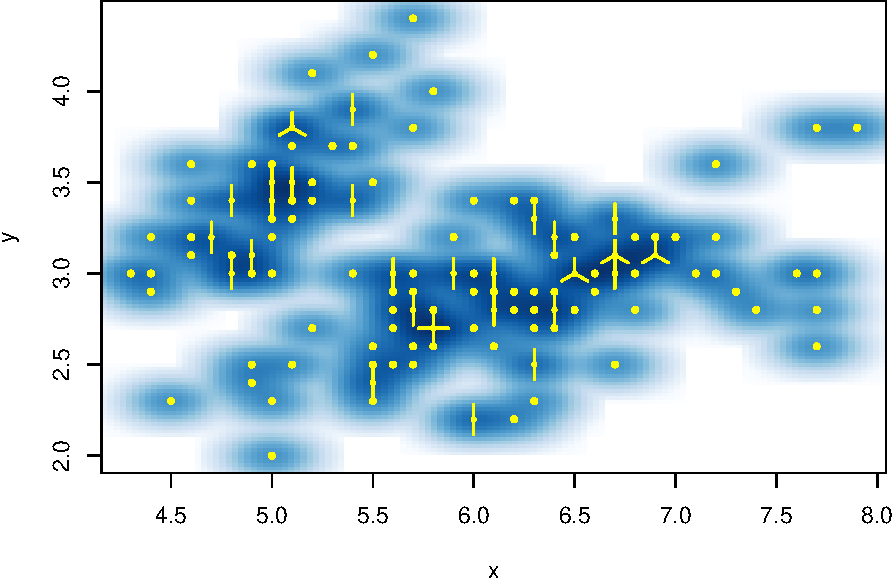
\includegraphics{2020-rstudio-conf-rmarkdown-demo_files/9/star-1} \end{center}

\end{CodeChunk}

\hypertarget{create-tables}{%
\subsection{Create tables}\label{create-tables}}

\hypertarget{a-simple-table}{%
\subsubsection{A simple table}\label{a-simple-table}}

\begin{CodeChunk}

\begin{CodeInput}
R> fit <- lm(y ~ x, data = dat)
R> tab <- coef(summary(fit))  # regression coefficients
R> knitr::kable(tab, caption = 'A simple table.')
\end{CodeInput}


Table: A simple table.

               Estimate   Std. Error   t value   Pr(>|t|)
------------  ---------  -----------  --------  ---------
(Intercept)       3.419        0.254     13.48      0.000
x                -0.062        0.043     -1.44      0.152

\end{CodeChunk}

\hypertarget{inline-code}{%
\subsection{Inline code}\label{inline-code}}

\hypertarget{the-model}{%
\subsubsection{The model}\label{the-model}}

The fitted model is: \[Y = 3.419 + -0.062X\]

\hypertarget{other-features}{%
\section{Other features}\label{other-features}}

\hypertarget{figure-caption}{%
\subsection{Figure caption}\label{figure-caption}}

You can also add captions and numbers to figures. See Figure
@ref(fig:pie) for example.

\begin{CodeChunk}

\begin{CodeInput}
R> par(mar = c(0, 1, 0, 1))
R> pie(
R+   c(280, 60, 20),
R+   c('Sky', 'Sunny side of pyramid', 'Shady side of pyramid'),
R+   col = c('#0292D8', '#F7EA39', '#C4B632'),
R+   init.angle = -50, border = NA
R+ )
\end{CodeInput}
\begin{figure}

{\centering 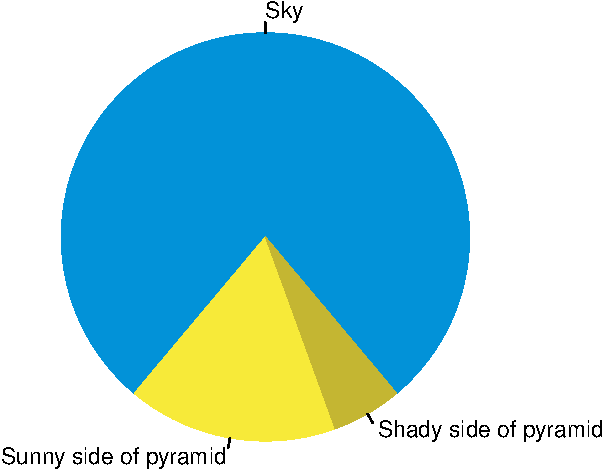
\includegraphics{2020-rstudio-conf-rmarkdown-demo_files/9/pie-1} 

}

\caption[My favorite pie chart]{My favorite pie chart.}\label{fig:pie}
\end{figure}
\end{CodeChunk}

\hypertarget{dynamic-content}{%
\subsection{Dynamic content}\label{dynamic-content}}

\hypertarget{animation}{%
\subsubsection{Animation}\label{animation}}

\begin{CodeChunk}

\begin{CodeInput}
R> par(mar = c(0, 1, 0, 1))
R> a = sample(0:359, 1)
R> for (i in 1:2) {
R+   pie(c(i %% 2, 6), col = c('red', 'yellow'), labels = NA,
R+       init.angle = a)
R+ }
\end{CodeInput}


\begin{center}\animategraphics[,controls,loop]{1}{2020-rstudio-conf-rmarkdown-demo_files/9/pacman-}{1}{2}\end{center}

\end{CodeChunk}

\hypertarget{leaflet-maps}{%
\subsubsection{Leaflet maps}\label{leaflet-maps}}

\begin{CodeChunk}

\begin{CodeInput}
R> library(leaflet)
R> leaflet() %>% addTiles() %>% setView(-122.410951, 37.7858188, zoom = 19)
\end{CodeInput}
<!--html_preserve--><div id="htmlwidget-68bd882e55ac8756f842" style="width:100%;height:264.6px;" class="leaflet html-widget"></div>
<script type="application/json" data-for="htmlwidget-68bd882e55ac8756f842">{"x":{"options":{"crs":{"crsClass":"L.CRS.EPSG3857","code":null,"proj4def":null,"projectedBounds":null,"options":{}}},"calls":[{"method":"addTiles","args":["//{s}.tile.openstreetmap.org/{z}/{x}/{y}.png",null,null,{"minZoom":0,"maxZoom":18,"tileSize":256,"subdomains":"abc","errorTileUrl":"","tms":false,"noWrap":false,"zoomOffset":0,"zoomReverse":false,"opacity":1,"zIndex":1,"detectRetina":false,"attribution":"&copy; <a href=\"http://openstreetmap.org\">OpenStreetMap<\/a> contributors, <a href=\"http://creativecommons.org/licenses/by-sa/2.0/\">CC-BY-SA<\/a>"}]}],"setView":[[37.7858188,-122.410951],19,[]]},"evals":[],"jsHooks":[]}</script><!--/html_preserve-->\end{CodeChunk}

\hypertarget{datatables}{%
\subsubsection{DataTables}\label{datatables}}

\begin{CodeChunk}

\begin{CodeInput}
R> DT::datatable(iris)
\end{CodeInput}
<!--html_preserve--><div id="htmlwidget-03524ef353d13e0161bc" style="width:100%;height:auto;" class="datatables html-widget"></div>
<script type="application/json" data-for="htmlwidget-03524ef353d13e0161bc">{"x":{"filter":"none","data":[["1","2","3","4","5","6","7","8","9","10","11","12","13","14","15","16","17","18","19","20","21","22","23","24","25","26","27","28","29","30","31","32","33","34","35","36","37","38","39","40","41","42","43","44","45","46","47","48","49","50","51","52","53","54","55","56","57","58","59","60","61","62","63","64","65","66","67","68","69","70","71","72","73","74","75","76","77","78","79","80","81","82","83","84","85","86","87","88","89","90","91","92","93","94","95","96","97","98","99","100","101","102","103","104","105","106","107","108","109","110","111","112","113","114","115","116","117","118","119","120","121","122","123","124","125","126","127","128","129","130","131","132","133","134","135","136","137","138","139","140","141","142","143","144","145","146","147","148","149","150"],[5.1,4.9,4.7,4.6,5,5.4,4.6,5,4.4,4.9,5.4,4.8,4.8,4.3,5.8,5.7,5.4,5.1,5.7,5.1,5.4,5.1,4.6,5.1,4.8,5,5,5.2,5.2,4.7,4.8,5.4,5.2,5.5,4.9,5,5.5,4.9,4.4,5.1,5,4.5,4.4,5,5.1,4.8,5.1,4.6,5.3,5,7,6.4,6.9,5.5,6.5,5.7,6.3,4.9,6.6,5.2,5,5.9,6,6.1,5.6,6.7,5.6,5.8,6.2,5.6,5.9,6.1,6.3,6.1,6.4,6.6,6.8,6.7,6,5.7,5.5,5.5,5.8,6,5.4,6,6.7,6.3,5.6,5.5,5.5,6.1,5.8,5,5.6,5.7,5.7,6.2,5.1,5.7,6.3,5.8,7.1,6.3,6.5,7.6,4.9,7.3,6.7,7.2,6.5,6.4,6.8,5.7,5.8,6.4,6.5,7.7,7.7,6,6.9,5.6,7.7,6.3,6.7,7.2,6.2,6.1,6.4,7.2,7.4,7.9,6.4,6.3,6.1,7.7,6.3,6.4,6,6.9,6.7,6.9,5.8,6.8,6.7,6.7,6.3,6.5,6.2,5.9],[3.5,3,3.2,3.1,3.6,3.9,3.4,3.4,2.9,3.1,3.7,3.4,3,3,4,4.4,3.9,3.5,3.8,3.8,3.4,3.7,3.6,3.3,3.4,3,3.4,3.5,3.4,3.2,3.1,3.4,4.1,4.2,3.1,3.2,3.5,3.6,3,3.4,3.5,2.3,3.2,3.5,3.8,3,3.8,3.2,3.7,3.3,3.2,3.2,3.1,2.3,2.8,2.8,3.3,2.4,2.9,2.7,2,3,2.2,2.9,2.9,3.1,3,2.7,2.2,2.5,3.2,2.8,2.5,2.8,2.9,3,2.8,3,2.9,2.6,2.4,2.4,2.7,2.7,3,3.4,3.1,2.3,3,2.5,2.6,3,2.6,2.3,2.7,3,2.9,2.9,2.5,2.8,3.3,2.7,3,2.9,3,3,2.5,2.9,2.5,3.6,3.2,2.7,3,2.5,2.8,3.2,3,3.8,2.6,2.2,3.2,2.8,2.8,2.7,3.3,3.2,2.8,3,2.8,3,2.8,3.8,2.8,2.8,2.6,3,3.4,3.1,3,3.1,3.1,3.1,2.7,3.2,3.3,3,2.5,3,3.4,3],[1.4,1.4,1.3,1.5,1.4,1.7,1.4,1.5,1.4,1.5,1.5,1.6,1.4,1.1,1.2,1.5,1.3,1.4,1.7,1.5,1.7,1.5,1,1.7,1.9,1.6,1.6,1.5,1.4,1.6,1.6,1.5,1.5,1.4,1.5,1.2,1.3,1.4,1.3,1.5,1.3,1.3,1.3,1.6,1.9,1.4,1.6,1.4,1.5,1.4,4.7,4.5,4.9,4,4.6,4.5,4.7,3.3,4.6,3.9,3.5,4.2,4,4.7,3.6,4.4,4.5,4.1,4.5,3.9,4.8,4,4.9,4.7,4.3,4.4,4.8,5,4.5,3.5,3.8,3.7,3.9,5.1,4.5,4.5,4.7,4.4,4.1,4,4.4,4.6,4,3.3,4.2,4.2,4.2,4.3,3,4.1,6,5.1,5.9,5.6,5.8,6.6,4.5,6.3,5.8,6.1,5.1,5.3,5.5,5,5.1,5.3,5.5,6.7,6.9,5,5.7,4.9,6.7,4.9,5.7,6,4.8,4.9,5.6,5.8,6.1,6.4,5.6,5.1,5.6,6.1,5.6,5.5,4.8,5.4,5.6,5.1,5.1,5.9,5.7,5.2,5,5.2,5.4,5.1],[0.2,0.2,0.2,0.2,0.2,0.4,0.3,0.2,0.2,0.1,0.2,0.2,0.1,0.1,0.2,0.4,0.4,0.3,0.3,0.3,0.2,0.4,0.2,0.5,0.2,0.2,0.4,0.2,0.2,0.2,0.2,0.4,0.1,0.2,0.2,0.2,0.2,0.1,0.2,0.2,0.3,0.3,0.2,0.6,0.4,0.3,0.2,0.2,0.2,0.2,1.4,1.5,1.5,1.3,1.5,1.3,1.6,1,1.3,1.4,1,1.5,1,1.4,1.3,1.4,1.5,1,1.5,1.1,1.8,1.3,1.5,1.2,1.3,1.4,1.4,1.7,1.5,1,1.1,1,1.2,1.6,1.5,1.6,1.5,1.3,1.3,1.3,1.2,1.4,1.2,1,1.3,1.2,1.3,1.3,1.1,1.3,2.5,1.9,2.1,1.8,2.2,2.1,1.7,1.8,1.8,2.5,2,1.9,2.1,2,2.4,2.3,1.8,2.2,2.3,1.5,2.3,2,2,1.8,2.1,1.8,1.8,1.8,2.1,1.6,1.9,2,2.2,1.5,1.4,2.3,2.4,1.8,1.8,2.1,2.4,2.3,1.9,2.3,2.5,2.3,1.9,2,2.3,1.8],["setosa","setosa","setosa","setosa","setosa","setosa","setosa","setosa","setosa","setosa","setosa","setosa","setosa","setosa","setosa","setosa","setosa","setosa","setosa","setosa","setosa","setosa","setosa","setosa","setosa","setosa","setosa","setosa","setosa","setosa","setosa","setosa","setosa","setosa","setosa","setosa","setosa","setosa","setosa","setosa","setosa","setosa","setosa","setosa","setosa","setosa","setosa","setosa","setosa","setosa","versicolor","versicolor","versicolor","versicolor","versicolor","versicolor","versicolor","versicolor","versicolor","versicolor","versicolor","versicolor","versicolor","versicolor","versicolor","versicolor","versicolor","versicolor","versicolor","versicolor","versicolor","versicolor","versicolor","versicolor","versicolor","versicolor","versicolor","versicolor","versicolor","versicolor","versicolor","versicolor","versicolor","versicolor","versicolor","versicolor","versicolor","versicolor","versicolor","versicolor","versicolor","versicolor","versicolor","versicolor","versicolor","versicolor","versicolor","versicolor","versicolor","versicolor","virginica","virginica","virginica","virginica","virginica","virginica","virginica","virginica","virginica","virginica","virginica","virginica","virginica","virginica","virginica","virginica","virginica","virginica","virginica","virginica","virginica","virginica","virginica","virginica","virginica","virginica","virginica","virginica","virginica","virginica","virginica","virginica","virginica","virginica","virginica","virginica","virginica","virginica","virginica","virginica","virginica","virginica","virginica","virginica","virginica","virginica","virginica","virginica","virginica","virginica"]],"container":"<table class=\"display\">\n  <thead>\n    <tr>\n      <th> <\/th>\n      <th>Sepal.Length<\/th>\n      <th>Sepal.Width<\/th>\n      <th>Petal.Length<\/th>\n      <th>Petal.Width<\/th>\n      <th>Species<\/th>\n    <\/tr>\n  <\/thead>\n<\/table>","options":{"columnDefs":[{"className":"dt-right","targets":[1,2,3,4]},{"orderable":false,"targets":0}],"order":[],"autoWidth":false,"orderClasses":false}},"evals":[],"jsHooks":[]}</script><!--/html_preserve-->\end{CodeChunk}

\bibliography{R-packages.bib}


\end{document}

